\documentclass[11pt]{article}
\usepackage[margin=1in]{geometry}
\usepackage{booktabs}
\usepackage{graphicx}
\usepackage{microtype}
\usepackage[hidelinks]{hyperref}

\newcommand{\FactAcc}{1.0}
\newcommand{\CovDetect}{3/3}
\newcommand{\GndDetect}{3/3}
\newcommand{\LinDetect}{1/3}


\title{\vspace{-2em}\textbf{Is the LLM judge fair?}}
\author{arxivkg · evaluation · judge validity}
\date{}

\begin{document}
\maketitle
\vspace{-2em}

\section*{What we did}
Quality verdicts rest on an LLM judge (Gemma-4-26B): 4 axes + an order-debiased pairwise. We test it
against \textbf{ground truth} three ways: (1) \textbf{known facts} --- 24 claims about famous papers
(true / false-topic / false-subtle), accept the true, reject the false; (2) \textbf{degradations} ---
prefer a full review over truncated (coverage), citation-stripped (grounding), chronology-corrupted
(lineage) variants; (3) \textbf{bias} --- identical inputs must tie (position), a content-free padded
variant must not win (verbosity). The chronology corruption reverse-maps years so the prose
contradicts the dates --- an internal inconsistency caught by arithmetic, independent of the judge's
stale ``now'' (today's date is also injected).

\section*{Results}
\textbf{Known-fact accuracy: \FactAcc} (n=24) --- it rejects even subtle method-confusions
(``DDPM uses a GAN objective'' $\rightarrow$ no; ``Transformer relies on RNNs'' $\rightarrow$ no).
Coverage detection \CovDetect, grounding \GndDetect, lineage \LinDetect.

\begin{center}\begin{tabular}{lrrr}
\toprule
degradation & full & tie & variant \\
\midrule
identical & 0 & 3 & 0 \\
truncated-75 & 3 & 0 & 0 \\
truncated-50 & 3 & 0 & 0 \\
truncated-25 & 3 & 0 & 0 \\
citations-stripped & 3 & 0 & 0 \\
shuffled & 3 & 0 & 0 \\
chronology-corrupted & 1 & 2 & 0 \\
verbose-pad & 0 & 3 & 0 \\
\bottomrule
\end{tabular}
\end{center}
\begin{center}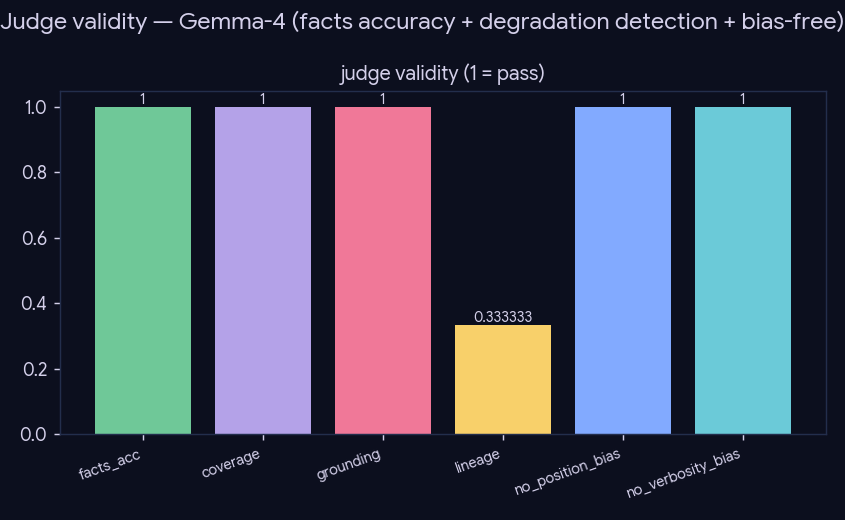
\includegraphics[width=0.85\textwidth]{../results/validity.png}\end{center}

Position bias \textbf{0/6 (clean)}; verbosity bias \textbf{none}.

\section*{Conclusion}
The judge is \textbf{valid and unbiased on the objective dimensions} --- perfect on factual ground
truth, catches coverage and grounding degradations at every level, no position or verbosity bias.
\textbf{Lineage is its weak axis} (catches genuine chronology corruption only sometimes; correctly
ignores cosmetic reordering). Rule for every downstream experiment: \textbf{trust grounding/coverage
and large effects; asterisk lineage and sub-noise-floor margins.} Caveat: small ground-truth set;
same-family judging, but a cross-family agreement check found no systematic self-preference.

\end{document}
